\documentclass[12pt,a4paper]{article}
\usepackage[utf8]{inputenc}
\usepackage[T1]{fontenc}
\usepackage[margin=1in]{geometry}
\usepackage{graphicx,float,amsmath,amsfonts,amssymb}
\usepackage{fancyhdr,listings,xcolor,caption,subcaption,hyperref,booktabs,multirow}
\usepackage{lmodern,microtype}
\definecolor{primaryblue}{RGB}{0,51,102}
\definecolor{secondaryblue}{RGB}{0,102,204}
\definecolor{darkgray}{RGB}{64,64,64}
\lstdefinestyle{matlabstyle}{language=Matlab,basicstyle=\ttfamily\footnotesize,
keywordstyle=\color{blue},commentstyle=\color{green!40!black},stringstyle=\color{red},
breaklines=true,keepspaces=true,numbers=left,numberstyle=\tiny\color{gray},
numbersep=5pt,showstringspaces=false,tabsize=2,frame=single,
rulecolor=\color{primaryblue!25},backgroundcolor=\color{primaryblue!3},
xleftmargin=1em,framexleftmargin=.5em,aboveskip=7pt,belowskip=7pt}
\lstset{style=matlabstyle}
\hypersetup{colorlinks=true,linkcolor=primaryblue,urlcolor=secondaryblue,citecolor=primaryblue,
pdftitle={3D Aircraft Tracking with an Extended Kalman Filter},pdfauthor={Kuruppuarachchi K.A.R.R}}
\pagestyle{fancy}\fancyhf{}
\fancyhead[L]{\small EN4594 -- Autonomous Systems}
\fancyhead[R]{\small EKF Mini Project}
\fancyfoot[C]{\thepage}
\setlength{\headheight}{16pt}
\setlength{\parindent}{0pt}\setlength{\parskip}{5pt}
\captionsetup{font=small,labelfont=bf}
\graphicspath{{figures/}}
\setcounter{topnumber}{3}
\renewcommand{\topfraction}{.92}\renewcommand{\bottomfraction}{.9}
\renewcommand{\textfraction}{.06}\renewcommand{\floatpagefraction}{.75}
\emergencystretch=2em
% User-supplied identity. Edit the date when the report is submitted.
\newcommand{\StudentName}{Kuruppuarachchi K.A.R.R}
\newcommand{\ModuleCode}{EN4594}
\newcommand{\ModuleTitle}{Autonomous Systems}
\newcommand{\SubmissionDate}{11 November 2026}

\begin{document}
\hypersetup{pageanchor=false}
\begin{titlepage}
\centering\vspace*{0.5cm}
% Official wordmark has transparent white lettering; backing preserves contrast.
\colorbox{primaryblue}{
\includegraphics[width=0.54\textwidth]{University_of_Moratuwa_logo.png}}
\vspace{1cm}

{\sffamily\Large\bfseries\color{primaryblue} UNIVERSITY OF MORATUWA\par}
\vspace{0.3cm}
{\sffamily\large\color{secondaryblue} Department of Electronic \& Telecommunication Engineering\par}
\vspace{1.1cm}
{\sffamily\Huge\bfseries\color{primaryblue} \ModuleCode\par}
\vspace{0.3cm}
{\sffamily\LARGE\bfseries\color{secondaryblue} \ModuleTitle\par}
\vspace{0.9cm}
{\sffamily\Large\bfseries\color{darkgray} Mini Project\par}
\vspace{0.4cm}
{\sffamily\Large\bfseries\color{darkgray} Three-Dimensional Aircraft Tracking\par}
\vspace{0.2cm}
{\sffamily\large\color{darkgray} with an Extended Kalman Filter\par}
\vspace{0.3cm}
{\sffamily\normalsize\color{darkgray} Virtual-radar simulation and recorded-flight replay\par}
\vspace{1.1cm}
{\sffamily\large\bfseries\color{primaryblue} Submitted by:\par}
\vspace{0.4cm}
{\sffamily\normalsize\color{darkgray} \StudentName\par}
\vspace{1cm}
{\sffamily\normalsize\color{darkgray} Date of Submission: \SubmissionDate\par}
\vfill
{\sffamily\footnotesize\color{darkgray} 2022 Batch -- Semester 07\par}
\end{titlepage}
\hypersetup{pageanchor=true}
\pagenumbering{arabic}
\section{Introduction and simulation design}
Aircraft tracking requires an estimate of position and velocity from noisy observations. This project implements one Extended Kalman Filter (EKF) for a virtual radar measuring slant range, azimuth and elevation. A six-state model predicts three-dimensional motion, and a nonlinear update corrects it. The study first evaluates controlled simulations with known truth, then replays ten distinct recorded flights. Each run tracks one known target; detection, clutter and multi-target association are outside its scope.

\subsection{Controlled simulation scenarios}
Every deterministic scenario lasts 600~s with 1~s sampling. The initial position is $[10000,5000,2000]$~m, and velocity is $[100,20,0]$~m/s. Straight flight establishes noise suppression. The manoeuvre case turns at $1^\circ$/s from 180--240~s, then climbs at 3~m/s from 300--420~s. The outage case uses that manoeuvre and omits 21 observations from 200--220~s.
\begin{lstlisting}
cfg = tracking_config();
[t,truth] = generate_truth('dropout');
z = generate_radar(truth,cfg);
z(t>=200 & t<=220,:) = NaN;
out = run_filters(t,z,cfg);
[metrics,nees] = evaluate_tracking(truth,z,out,cfg);
\end{lstlisting}
This MATLAB excerpt uses truth only to create radar data and evaluate errors. The estimator receives timestamps, radar measurements and configuration; it cannot access the true trajectory. All filter calculations use metres, seconds and radians.

\subsection{Repeated tests and matched-model check}
Four scenarios are evaluated over 100 independent noise trials each: straight flight, turn/climb, outage and stochastic constant-velocity motion. The first three use fixed trajectories with independent radar noise. In the matched case, motion itself is sampled using the same $F,Q$ as the filter, allowing a controlled covariance-consistency check.

The 400 repeated simulation runs and expanded flight benchmarks are executed locally with the equivalent, previously numerically audited EKF. The original MATLAB Online runs supply the figures and implementation excerpts; additional MATLAB Online execution is not claimed. Simulation measurement seeds are 100000--100099; matched-motion seeds are 1000--1099. Process intensity is fixed at $q=1$ for the simulation study.

The evaluation reports position and velocity RMSE, plus innovation consistency. Initialization samples are excluded. During an outage, all-time error and observation-available error are distinguished because the raw radar has no measurements during the gap. The following sections explain the MATLAB model and update before presenting simulation results and then the flight datasets.
\clearpage
\section{Methodology: motion and radar models}
The state is $\mathbf{x}=[p_E,p_N,p_U,v_E,v_N,v_U]^T$. For interval $\Delta t$, the constant-velocity prediction is $\mathbf{x}_{k|k-1}=F_k\mathbf{x}_{k-1|k-1}$. Continuous white acceleration with intensity $q$ gives
\[
F=\begin{bmatrix}I&\Delta t I\\0&I\end{bmatrix},\qquad
Q=q\begin{bmatrix}\Delta t^3 I/3&\Delta t^2 I/2\\\Delta t^2 I/2&\Delta t I\end{bmatrix}.
\]
This follows from $\dot{\mathbf p}=\mathbf v$, $\dot{\mathbf v}=\mathbf w$, where $\mathbf w$ is white acceleration of spectral density $qI$:
\[
Q=\int_0^{\Delta t}\begin{bmatrix}\tau I\\I\end{bmatrix}
qI\begin{bmatrix}\tau I&I\end{bmatrix}\,d\tau.
\]
The integrals of $\tau^2$, $\tau$ and 1 give the three powers of $\Delta t$ above. Here $q$ has units m$^2$/s$^3$, not acceleration variance. Recompute $F,Q$ at every interval.
\begin{lstlisting}
I = eye(3);
F = [I dt*I; zeros(3) I];
Q = q*[dt^3/3*I dt^2/2*I; dt^2/2*I dt*I];
R = diag([50; 0.5*pi/180; 0.5*pi/180].^2);
\end{lstlisting}
For position $\mathbf{p}=(p_E,p_N,p_U)$, let $\rho=\sqrt{p_E^2+p_N^2}$ and $r=\|\mathbf{p}\|$. The radar function is $h(\mathbf{x})=[r,\operatorname{atan2}(p_N,p_E),\operatorname{atan2}(p_U,\rho)]^T$. Independent Gaussian noise has standard deviations 50~m in range and $0.5^\circ$ in both angles. Thus $\mathbf{z}=h(\mathbf{x}_{\rm ref})+\boldsymbol{\eta}$, with $\boldsymbol{\eta}\sim\mathcal{N}(0,R)$.

The EKF linearises at the predicted state: $h(\mathbf x)\approx h(\hat{\mathbf x}^{-})+H(\mathbf x-\hat{\mathbf x}^{-})$. Differentiation gives, for example, $\partial r/\partial p_E=p_E/r$ and $\partial a/\partial p_E=-p_N/\rho^2$. The MATLAB Jacobian is:
\begin{lstlisting}
p = x(1:3); rho = hypot(p(1),p(2)); r = norm(p);
valid = r >= cfg.min_range && rho >= cfg.min_rho;
h = [r; atan2(p(2),p(1)); atan2(p(3),rho)];
H = NaN(3,6);
if ~valid, return; end
H = [p'/r zeros(1,3);
    -p(2)/rho^2 p(1)/rho^2 0 zeros(1,3);
    -p(1)*p(3)/(r^2*rho) ...
    -p(2)*p(3)/(r^2*rho) rho/r^2 zeros(1,3)];
\end{lstlisting}
Velocity columns of $H$ are zero, but successive positions constrain velocity through $F$. At predicted $r<1$~m or $\rho<1$~m, the singular angular update is skipped. Accuracy still depends on linearisation and motion assumptions.
\clearpage
\section{Initialization from two radar observations}
A starting velocity is required before recursive prediction. Each of the first two radar observations is converted into Cartesian position. Its uncertainty is propagated using the conversion Jacobian, rather than assigning equal uncertainty to all position axes.
\begin{lstlisting}
% Within convert_radar(z,R):
r = z(1); a = z(2); e = z(3);
ca = cos(a); sa = sin(a); ce = cos(e); se = sin(e);
p = [r*ce*ca; r*ce*sa; r*se];
J = [ce*ca -r*ce*sa -r*se*ca;
     ce*sa  r*ce*ca -r*se*sa;
     se     0        r*ce];
C = J*R*J';
C = (C+C')/2;
\end{lstlisting}
Let these positions be $\mathbf{p}_1,\mathbf{p}_2$ with independent covariances $C_1,C_2$. The initial state at the second observation is $[\mathbf{p}_2^T,(\mathbf{p}_2-\mathbf{p}_1)^T/d]^T$, where $d=t_2-t_1$.
\begin{lstlisting}
[p1,C1] = convert_radar(z(1,:)',cfg.R);
[p2,C2] = convert_radar(z(2,:)',cfg.R);
d = t(2)-t(1);
x0 = [p2; (p2-p1)/d];
P0 = [C2 C2/d; C2/d (C1+C2)/d^2];
xe = x0; Pe = P0;
\end{lstlisting}
For independent measurement errors, $\operatorname{Cov}(\mathbf p_2,(\mathbf p_2-\mathbf p_1)/d)=C_2/d$. The same second position appears in both position and velocity. Omitting that correlation would misrepresent the uncertainty. The factor $1/d^2$ also explains why velocity initialization can be noisy when positions are closely spaced. Process uncertainty between the first two observations is omitted in this initialization approximation; long gaps and manoeuvres can make it overconfident.

\subsection{Input checks and scoring boundary}
\begin{lstlisting}
assert(all(isfinite(t)) && all(diff(t)>0));
present = all(isfinite(z),2);
missing = all(isnan(z),2);
assert(all(present | missing));
assert(all(z(present,1)>0));
assert(all(abs(z(present,3))<pi/2));
% First two observations must be present.
% Recursive updates and scored errors begin at row 3.
\end{lstlisting}
An absent radar observation is represented by an entire row of \texttt{NaN}. Partially missing observations are rejected. The first two rows initialize the state and are excluded from error statistics. The second observation is not reused as a corrective update, which avoids counting the same information twice.
\clearpage
\section{Recursive MATLAB implementation}
At each timestamp the EKF first predicts state and covariance, then applies a correction if a valid radar observation is available. The following excerpt contains the core of the implemented loop; output storage is included for reproducible plots and metrics.
\begin{lstlisting}
for k = 3:numel(t)
    dt = t(k)-t(k-1);
    [F,Q] = cv_model(dt,cfg.q);
    xe = F*xe;
    Pe = F*Pe*F' + Q;
    if present(k)
        [h,H,valid] = radar_model(xe,cfg);
        if valid
            v = z(k,:)'-h;
            v(2) = atan2(sin(v(2)),cos(v(2)));
            S = H*Pe*H' + cfg.R;
            K = (Pe*H')/S;
            nis(k) = v'*(S\v);
            xe = xe + K*v;
            A = eye(6)-K*H;
            Pe = A*Pe*A' + K*cfg.R*K';
        end
    end
    Pe = (Pe+Pe')/2;
    estimate(k,:) = xe';
    covariance(:,:,k) = Pe;
end
\end{lstlisting}
The innovation $\mathbf{v}=\mathbf{z}-h(\mathbf{x})$ compares measured and predicted radar coordinates. Azimuth is periodic, so its innovation is wrapped to $[-\pi,\pi]$; otherwise crossing the angular boundary can produce an artificial near-$2\pi$ correction. Elevation remains within its physical interval.

The matrix $S=HPH^T+R$ expresses predicted innovation uncertainty. The Kalman gain balances it against state uncertainty. MATLAB right division and backslash solve linear systems without explicitly forming matrix inverses. The Joseph covariance update $(I-KH)P(I-KH)^T+KRK^T$ reduces numerical loss of symmetry and positive semidefiniteness. Final symmetrization removes roundoff asymmetry.

During a missing observation, prediction continues and $Q$ increases uncertainty. There is no innovation or NIS for that row. When observations resume, the larger covariance allows stronger corrections. This maintains a track through an outage, although an unobserved turn cannot be recovered exactly from a constant-velocity model.

\textbf{Correctness checks.} Twenty-three automated checks cover analytical versus numerical Jacobians, correlated initialization, angle wrapping, irregular timing, outages and covariance validity. All 13 returned MATLAB runs also pass identical-observation state, covariance and metric checks within $10^{-7}+10^{-8}|\mathrm{reference}|$. These verify tested implementations, while the results below assess model effectiveness.
\clearpage
\section{Simulation results and scoring}
The first two observations initialize the filter and are excluded from scoring. For $N$ input rows, let $M=N-2$. Position RMSE is
\begin{equation}
\mathrm{RMSE}_{p}=\sqrt{\frac{1}{M}\sum_{k=3}^{N}\|\hat{\mathbf p}_k-\mathbf p_k\|^2}.
\end{equation}
Velocity RMSE uses the corresponding velocity vectors. The MATLAB scoring excerpt is:
\begin{lstlisting}
idx = (3:size(truth,1))';
e = out.ekf(idx,1:3)-truth(idx,1:3);
posRMSE = sqrt(mean(sum(e.^2,2)));
ev = out.ekf(idx,4:6)-truth(idx,4:6);
velRMSE = sqrt(mean(sum(ev.^2,2)));
meanNIS = mean(out.ekf_nis(isfinite(out.ekf_nis)));
\end{lstlisting}
\begin{table}[H]\centering\small
\begin{tabular}{lrrr}\toprule
Scenario & EKF position (m) & Raw position (m) & Velocity (m/s)\\\midrule
Straight & 125.20 & 561.77 & 7.18 \\
Turn/climb & 175.59 & 516.33 & 13.52 \\
Turn with outage & 215.93 & 520.14 & 15.32 \\
Matched stochastic CV & 141.39 & 555.49 & 9.74 \\
\bottomrule\end{tabular}
\caption{Local simulation evaluation: mean trial-level RMSE over 100 trials per scenario, $q=1$. EKF position includes outage rows; raw position uses only available observations.}
\end{table}
Straight flight achieves 77.7\% mean position-error reduction relative to raw observations. Turning increases error because the constant-velocity predictor cannot anticipate changing heading. For the outage case, the fair observed-time EKF RMSE is 174.85~m against raw 520.14~m; 215.93~m includes the missing-observation interval. Approximate 95\% intervals for mean position RMSE are 122.91--127.48~m (straight), 173.08--178.09~m (turn), and 212.67--219.20~m (outage). They describe noise-trial means, not bounds on every sample.

\subsection{Covariance consistency under matched motion}
NIS is $\mathbf v^TS^{-1}\mathbf v$, with nominal expectation 3 for three measurements. With exact six-state truth, NEES is $\mathbf e^TP^{-1}\mathbf e$, with expectation 6. At 600~s across 100 independent matched trials, mean NIS is 3.134 within approximate 95\% ensemble bounds $[2.539,3.499]$; mean NEES is 5.433 within $[5.340,6.698]$. This supports consistency at that tested time under matched assumptions, not during arbitrary manoeuvres.

The original MATLAB seed-42 position RMSE is 124.83~m for straight flight, 190.66~m for turn/climb, and 246.10~m for outage (191.76~m on observed rows). These are individual realizations; the table averages independent local trials. No second filter is implemented: raw converted radar points supply the unfiltered comparison.
\clearpage
\section{MATLAB plots: manoeuvre and radar outage}
\begin{figure}[H]\centering
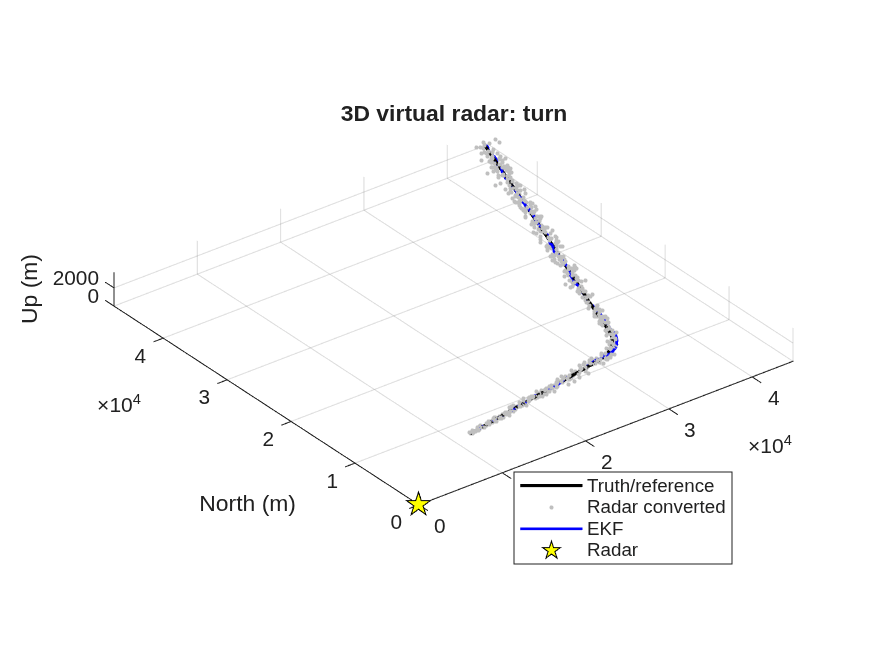
\includegraphics[width=.79\textwidth,height=.29\textheight,keepaspectratio]{matlab_turn_track.png}
\caption{Original MATLAB turn/climb trajectory. Black: simulated reference; grey: converted noisy radar; blue: EKF; star: radar at the origin. The MATLAB plot uses equal data-unit scaling; perspective affects its appearance.}
\end{figure}
The EKF follows the broad 3D path while suppressing measurement scatter. The track alone can hide errors of hundreds of metres because the full path extends tens of kilometres; error plots are needed to assess filtering quality.
\begin{figure}[H]\centering
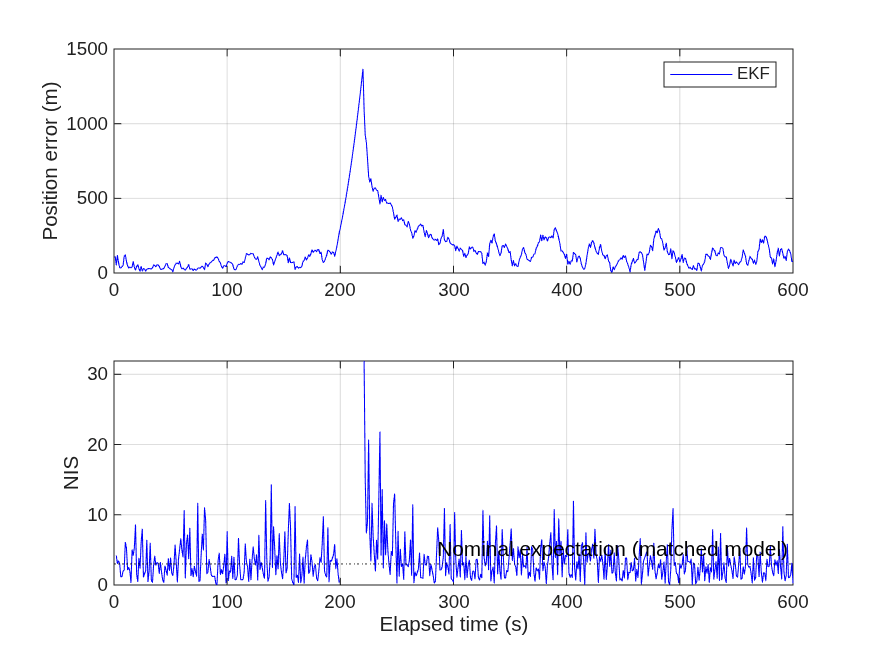
\includegraphics[width=.79\textwidth,height=.29\textheight,keepaspectratio]{matlab_dropout_errors.png}
\caption{Original MATLAB outage result: position error above and NIS below. Missing radar rows produce a break in the NIS history because no innovation is calculated.}
\end{figure}
The error increase during the turn and missing observations exposes the constant-velocity model's limitation. After measurements return, the filter corrects its predicted path. NIS excursions reveal that apparently smooth tracking does not always mean the assumed uncertainty matches the manoeuvre.
\clearpage
\section{Ten recorded-flight datasets and protocol}
Ten distinct aircraft trajectories come from the \texttt{traffic} sample collection: the original Belevingsvlucht/Texas tracks plus eight featured, calibration and survey examples. All ten files total 501,767 compressed bytes. Their positions are references, with synthetic radar observations.

\subsection{Coordinate preparation in MATLAB}
Degrees and feet are converted into approximate local east--north--up coordinates. Offsets keep the track away from the radar origin. Actual timestamp differences are preserved; no smoothing or interpolation is applied.
\begin{lstlisting}
T = readtable(path); t = T.elapsed_s;
lat = T.latitude_deg*pi/180; lon = T.longitude_deg*pi/180;
h = T.altitude_ft*0.3048;
east = 10000+6371000*cos(lat(1))*(lon-lon(1));
north = 5000+6371000*(lat-lat(1)); up = 2000+h-h(1);
truth = [east north up NaN(numel(t),3)];
\end{lstlisting}
Relative altitude has an unverified datum, and recorded velocities are not exact truth; replay velocity RMSE and NEES are therefore omitted.

\subsection{All-flight evaluation}
Every flight is tested in three fixed source-time windows: 0--10, 30--40 and 60--70 minutes. Each window uses 20 paired noise trials (seeds 3000--3019) at $q=1$ and $q=10$: 30 windows and 1,200 EKF runs. Earlier development used $q\in\{0.1,1,10,100\}$ on the first two flights' 0--10 minute windows (seeds 100--109), selecting 10 for both. The default 1 and selected 10 were frozen for the eight added flights. Both receive identical radar observations and unchanged $R$.
\begin{table}[H]\centering\footnotesize
\setlength{\tabcolsep}{4pt}
\begin{tabular}{llrrr}\toprule
Flight & Native counts$^*$ & $q=1$ (m) & $q=10$ (m) & Raw (m)\\\midrule
Belevingsvlucht & 550/549/586 & 292.3 & 163.5 & 377.8 \\
Texas & 42/20/26 & 563.7 & 405.9 & 461.9 \\
Dreamliner Boeing & 46/10/10 & 635.8 & 796.0 & 934.4 \\
Easter Rabbit & 61/61/61 & 145.2 & 145.3 & 189.8 \\
Qantas 747 & 61/61/61 & 400.4 & 203.6 & 191.2 \\
Thankyou & 61/61/61 & 229.5 & 188.1 & 242.4 \\
Brussels ILS & 121/121/121 & 365.0 & 195.9 & 258.8 \\
Cardiff & 121/121/121 & 341.6 & 163.7 & 176.4 \\
Kota Kinabalu & 121/121/121 & 414.2 & 211.4 & 238.7 \\
IGN Mercantour & 21/22/26 & 1905.8 & 1206.7 & 318.5 \\
\bottomrule\end{tabular}
\caption{All ten flights: mean trial-level 3D RMSE, equally averaged across the three windows. $^*$Counts correspond to window starts 0/30/60 minutes; two initialization rows per window are excluded from scores.}
\end{table}
At $q=10$, 8/10 flight means improve on raw error. Qantas 747 and IGN Mercantour remain worse; these failures limit conclusions from the original two flights.
\clearpage
\section{Results for every flight window}
The table covers every evaluated dataset window. Entries are means over 20 noise draws with settings fixed; no window or unsuccessful run has been omitted. All 1,200 runs retain finite states and valid covariance matrices within numerical tolerance. Every scored row receives its available radar update.
\begin{table}[H]\centering\footnotesize
\setlength{\tabcolsep}{3.5pt}
\renewcommand{\arraystretch}{1.02}
\begin{tabular}{llrrrrr}\toprule
Flight & Source min & Gap$^*$ & Raw (m) & $q=1$ (m) & $q=10$ (m) & NIS$^\dagger$\\\midrule
Belevingsvlucht & 0--10 & 5 & 378.4 & 257.0 & 163.7 & 3.71 \\
 & 30--40 & 4 & 545.9 & 329.3 & 202.8 & 4.07 \\
 & 60--70 & 3 & 209.1 & 290.7 & 123.9 & 3.83 \\
\addlinespace[2pt]
Texas & 0--10 & 35 & 358.9 & 287.0 & 287.1 & 3.45 \\
 & 30--40 & 46 & 527.9 & 664.2 & 469.5 & 6.20 \\
 & 60--70 & 60 & 499.0 & 739.9 & 461.2 & 5.40 \\
\addlinespace[2pt]
Dreamliner Boeing & 0--10 & 290 & 150.9 & 144.1 & 157.2 & 3.31 \\
 & 30--40 & 67 & 1295.2 & 870.5 & 1094.5 & 1.54 \\
 & 60--70 & 64 & 1357.0 & 893.0 & 1136.3 & 1.13 \\
\addlinespace[2pt]
Easter Rabbit & 0--10 & 10 & 177.1 & 126.4 & 138.1 & 2.12 \\
 & 30--40 & 10 & 252.7 & 184.6 & 182.2 & 2.74 \\
 & 60--70 & 10 & 139.6 & 124.7 & 115.5 & 2.44 \\
\addlinespace[2pt]
Qantas 747 & 0--10 & 10 & 147.6 & 101.2 & 120.9 & 1.87 \\
 & 30--40 & 10 & 172.7 & 445.6 & 198.5 & 12.66 \\
 & 60--70 & 10 & 253.5 & 654.3 & 291.5 & 16.89 \\
\addlinespace[2pt]
Thankyou & 0--10 & 10 & 168.2 & 210.4 & 144.0 & 5.09 \\
 & 30--40 & 10 & 238.6 & 225.1 & 188.8 & 3.98 \\
 & 60--70 & 10 & 320.5 & 253.0 & 231.7 & 3.97 \\
\addlinespace[2pt]
Brussels ILS & 0--10 & 5 & 263.9 & 394.7 & 193.9 & 4.54 \\
 & 30--40 & 5 & 278.3 & 394.0 & 206.4 & 4.45 \\
 & 60--70 & 5 & 234.1 & 306.4 & 187.3 & 8.08 \\
\addlinespace[2pt]
Cardiff & 0--10 & 5 & 177.8 & 367.1 & 174.3 & 7.66 \\
 & 30--40 & 5 & 187.4 & 440.6 & 182.9 & 6.43 \\
 & 60--70 & 5 & 163.9 & 217.2 & 133.8 & 4.41 \\
\addlinespace[2pt]
Kota Kinabalu & 0--10 & 5 & 286.5 & 516.2 & 259.7 & 6.87 \\
 & 30--40 & 5 & 257.1 & 413.4 & 216.6 & 8.81 \\
 & 60--70 & 5 & 172.4 & 313.0 & 158.0 & 9.00 \\
\addlinespace[2pt]
IGN Mercantour & 0--10 & 219 & 502.9 & 4932.3 & 3182.8 & 82.91 \\
 & 30--40 & 39 & 203.2 & 383.0 & 202.8 & 9.21 \\
 & 60--70 & 41 & 249.4 & 402.0 & 234.4 & 9.74 \\
\bottomrule\end{tabular}
\caption{All 30 local replay tests. $^*$Maximum native gap in seconds. $^\dagger$Mean NIS at $q=10$; its nominal matched-model expectation is 3. The RMSE entries are trial means, not pooled sample RMSEs.}
\end{table}
At $q=10$, 26/30 windows improve on raw observations, and 24/30 improve on $q=1$. Nevertheless, the equally weighted ten-flight mean is 368.01~m, above raw 338.99~m; at $q=1$ it is 529.36~m. The large IGN Mercantour error strongly affects this average. The 219~s gap coincides with substantial post-gap tracking error; numerical covariance validity alone does not establish tracking accuracy.

Vertical RMSE increases in 29/30 windows when $q$ rises. Sparse Dreamliner windows have only eight scored rows and NIS below 3. Repeated noise trials do not establish population-wide or between-observation accuracy.
\clearpage
\section{MATLAB illustrations of recorded-flight replay}
\begin{figure}[H]\centering
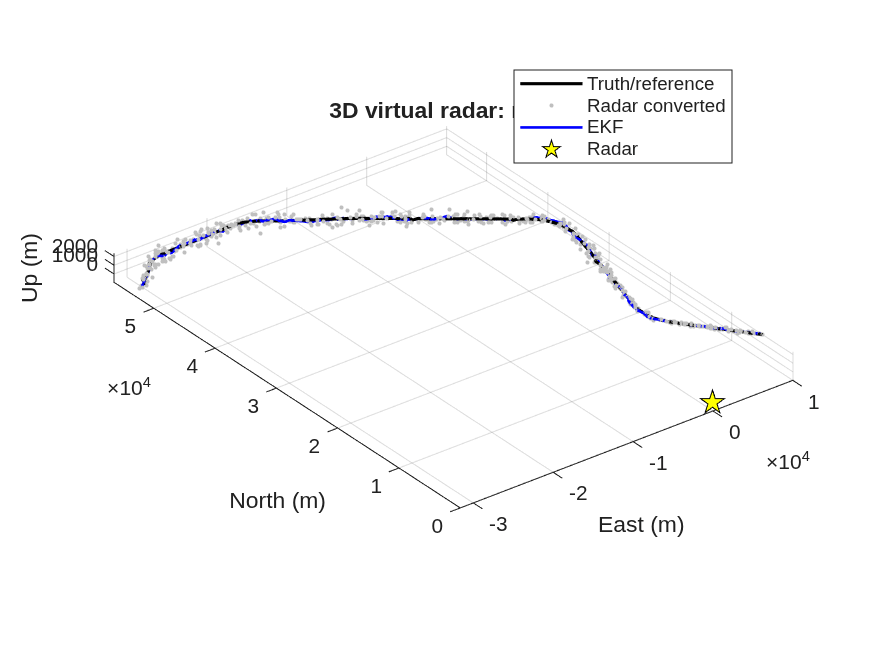
\includegraphics[width=.79\textwidth,height=.29\textheight,keepaspectratio]{matlab_belevingsvlucht_track.png}
\caption{Original MATLAB Belevingsvlucht 30--40 minute replay, $q=10$, seed 2000. The recorded-reference track is black, converted virtual radar grey, and the EKF blue.}
\end{figure}
This earlier MATLAB realization gives 191.92~m position RMSE and mean NIS 4.15. The local 20-trial mean for the same window is 202.83~m. A single image illustrates behaviour; it does not replace the repeated-trial evidence or depict every added flight.
\begin{figure}[H]\centering
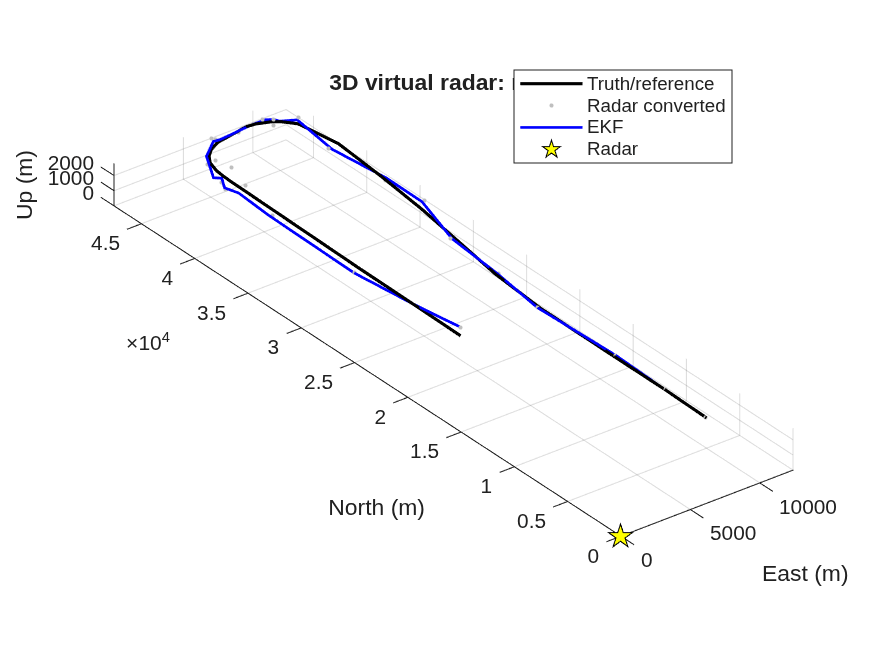
\includegraphics[width=.79\textwidth,height=.29\textheight,keepaspectratio]{matlab_texas_track.png}
\caption{Original MATLAB Texas 60--70 minute replay, $q=10$, seed 2000. Position RMSE is 365.45~m and mean NIS 5.30. Both figures are unchanged MATLAB outputs, separate from the new local benchmark.}
\end{figure}
Texas is sparser: 26 observations in this window, with a maximum gap of 60~s. Connecting lines add no observations and do not establish the actual intervening path. Its 20-trial mean RMSE is 461.20~m. Relative height has an unverified datum; these views demonstrate virtual-radar replay rather than certified physical radar performance.
\clearpage
\section{Discussion and conclusion}
\subsection{What the simulations establish}
The EKF combines nonlinear radar observations with a motion predictor to estimate position and velocity, reduce noise and preserve a predicted track during outages. Four hundred simulation runs distinguish typical behaviour from one realization. The matched-motion test supports final-time covariance consistency; turns and outages expose mismatch when the predictor cannot represent acceleration.

\subsection{What changes after testing ten flights}
The broader study is less favourable than the original two-flight demonstration. A larger $q$ improves 8/10 flight means and 24/30 windows, yet loses to raw measurements in four windows. IGN Mercantour's first window has severe post-gap errors. Motion mismatch and measurement linearisation can both contribute; the experiment does not isolate one cause or establish the source reference's accuracy.

Dreamliner Boeing shows the opposite tuning preference: increasing $q$ follows sparse noisy measurements more strongly and worsens all three window means. Easter Rabbit changes only marginally overall. Qantas 747 improves relative to $q=1$ yet loses to raw observations in two windows. A universal claim that larger process noise improves tracking is unsupported.

Equal weighting prevents dense tracks dominating the macro score, but difficult flights strongly influence it. Angular noise produces transverse error approximately $r\sigma_\theta$, so geometry also changes raw error. These selected references and repeated noise draws do not represent all air traffic.

\subsection{A justified next improvement}
The practical contribution combines 3D radar geometry, prediction through outages, native irregular sampling and a fixed-setting test on unseen flights. Numerical safeguards support this application; the EKF itself is established. The measured axis tradeoff motivates this untested extension:
\begin{lstlisting}
D = diag([qHorizontal qHorizontal qVertical]);
Q = [dt^3/3*D dt^2/2*D; dt^2/2*D dt*D];
\end{lstlisting}
It needs development-only tuning and fresh-flight evaluation. Long-gap recovery also needs explicit testing before operational use.

\subsection{Conclusion}
The 3D EKF achieves strong simulated noise reduction and improves on raw observations in most recorded-flight windows. The expanded 1,200-run study also reveals substantial failures, sparse-observation sensitivity and increased vertical error at larger $q$. Motion modelling and uncertainty selection remain critical to effectiveness.
\end{document}
